%%%%%%%%%%%%%%%%%%%%%%%%%%%%%%%%%%%%%%%%%
% Lachaise Assignment
% LaTeX Template
% Version 1.0 (26/6/2018)
%
% This template originates from:
% http://www.LaTeXTemplates.com
%
% Authors:
% Marion Lachaise & François Févotte
% Vel (vel@LaTeXTemplates.com)
%
% License:
% CC BY-NC-SA 3.0 (http://creativecommons.org/licenses/by-nc-sa/3.0/)
% 
%%%%%%%%%%%%%%%%%%%%%%%%%%%%%%%%%%%%%%%%%

%----------------------------------------------------------------------------------------
%	PACKAGES AND OTHER DOCUMENT CONFIGURATIONS
%----------------------------------------------------------------------------------------

\documentclass{article}

\usepackage{dirtree}
\usepackage{hyperref}
\usepackage{comment}
\usepackage{caption}
\usepackage{subcaption}
\usepackage{fancyvrb}
%\usepackage{enumitem}
%\usepackage{upquote,textcomp} % needed to fix single quotes in verbatium mode

%%%%%%%%%%%%%%%%%%%%%%%%%%%%%%%%%%%%%%%%%
% Lachaise Assignment
% Structure Specification File
% Version 1.0 (26/6/2018)
%
% This template originates from:
% http://www.LaTeXTemplates.com
%
% Authors:
% Marion Lachaise & François Févotte
% Vel (vel@LaTeXTemplates.com)
%
% License:
% CC BY-NC-SA 3.0 (http://creativecommons.org/licenses/by-nc-sa/3.0/)
% 
%%%%%%%%%%%%%%%%%%%%%%%%%%%%%%%%%%%%%%%%%

%----------------------------------------------------------------------------------------
%	PACKAGES AND OTHER DOCUMENT CONFIGURATIONS
%----------------------------------------------------------------------------------------

\usepackage{amsmath,amsfonts,stmaryrd,amssymb} % Math packages

\usepackage{enumerate} % Custom item numbers for enumerations

\usepackage[ruled]{algorithm2e} % Algorithms

\usepackage[framemethod=tikz]{mdframed} % Allows defining custom boxed/framed environments

\usepackage{listings} % File listings, with syntax highlighting
\lstset{
	basicstyle=\ttfamily, % Typeset listings in monospace font
}

%----------------------------------------------------------------------------------------
%	DOCUMENT MARGINS
%----------------------------------------------------------------------------------------

\usepackage{geometry} % Required for adjusting page dimensions and margins

\geometry{
	paper=a4paper, % Paper size, change to letterpaper for US letter size
	top=2.5cm, % Top margin
	bottom=3cm, % Bottom margin
	left=2.5cm, % Left margin
	right=2.5cm, % Right margin
	headheight=14pt, % Header height
	footskip=1.5cm, % Space from the bottom margin to the baseline of the footer
	headsep=1.2cm, % Space from the top margin to the baseline of the header
	%showframe, % Uncomment to show how the type block is set on the page
}

%----------------------------------------------------------------------------------------
%	FONTS
%----------------------------------------------------------------------------------------

\usepackage[utf8]{inputenc} % Required for inputting international characters
\usepackage[T1]{fontenc} % Output font encoding for international characters

\usepackage{XCharter} % Use the XCharter fonts

%----------------------------------------------------------------------------------------
%	COMMAND LINE ENVIRONMENT
%----------------------------------------------------------------------------------------

% Usage:
% \begin{commandline}
%	\begin{verbatim}
%		$ ls
%		
%		Applications	Desktop	...
%	\end{verbatim}
% \end{commandline}

\mdfdefinestyle{commandline}{
	leftmargin=10pt,
	rightmargin=10pt,
	innerleftmargin=15pt,
	middlelinecolor=black!50!white,
	middlelinewidth=2pt,
	frametitlerule=false,
	backgroundcolor=black!5!white,
	frametitle={Command Line},
	frametitlefont={\normalfont\sffamily\color{white}\hspace{-1em}},
	frametitlebackgroundcolor=black!50!white,
	nobreak,
}

% Define a custom environment for command-line snapshots
\newenvironment{commandline}{
	\medskip
	\begin{mdframed}[style=commandline]
}{
	\end{mdframed}
	\medskip
}

%----------------------------------------------------------------------------------------
%	FILE CONTENTS ENVIRONMENT
%----------------------------------------------------------------------------------------

% Usage:
% \begin{file}[optional filename, defaults to "File"]
%	File contents, for example, with a listings environment
% \end{file}

\mdfdefinestyle{file}{
	innertopmargin=1.6\baselineskip,
	innerbottommargin=0.8\baselineskip,
	topline=false, bottomline=false,
	leftline=false, rightline=false,
	leftmargin=2cm,
	rightmargin=2cm,
	singleextra={%
		\draw[fill=black!10!white](P)++(0,-1.2em)rectangle(P-|O);
		\node[anchor=north west]
		at(P-|O){\ttfamily\mdfilename};
		%
		\def\l{3em}
		\draw(O-|P)++(-\l,0)--++(\l,\l)--(P)--(P-|O)--(O)--cycle;
		\draw(O-|P)++(-\l,0)--++(0,\l)--++(\l,0);
	},
	nobreak,
}

% Define a custom environment for file contents
\newenvironment{file}[1][File]{ % Set the default filename to "File"
	\medskip
	\newcommand{\mdfilename}{#1}
	\begin{mdframed}[style=file]
}{
	\end{mdframed}
	\medskip
}

%----------------------------------------------------------------------------------------
%	NUMBERED QUESTIONS ENVIRONMENT
%----------------------------------------------------------------------------------------

% Usage:
% \begin{question}[optional title]
%	Question contents
% \end{question}

\mdfdefinestyle{question}{
	innertopmargin=1.2\baselineskip,
	innerbottommargin=0.8\baselineskip,
	roundcorner=5pt,
	nobreak,
	singleextra={%
		\draw(P-|O)node[xshift=1em,anchor=west,fill=white,draw,rounded corners=5pt]{%
		Question \theQuestion\questionTitle};
	},
}

\newcounter{Question} % Stores the current question number that gets iterated with each new question

% Define a custom environment for numbered questions
\newenvironment{question}[1][\unskip]{
	\bigskip
	\stepcounter{Question}
	\newcommand{\questionTitle}{~#1}
	\begin{mdframed}[style=question]
}{
	\end{mdframed}
	\medskip
}

%----------------------------------------------------------------------------------------
%	WARNING TEXT ENVIRONMENT
%----------------------------------------------------------------------------------------

% Usage:
% \begin{warn}[optional title, defaults to "Warning:"]
%	Contents
% \end{warn}

\mdfdefinestyle{warning}{
	topline=false, bottomline=false,
	leftline=false, rightline=false,
	nobreak,
	singleextra={%
		\draw(P-|O)++(-0.5em,0)node(tmp1){};
		\draw(P-|O)++(0.5em,0)node(tmp2){};
		\fill[black,rotate around={45:(P-|O)}](tmp1)rectangle(tmp2);
		\node at(P-|O){\color{white}\scriptsize\bf !};
		\draw[very thick](P-|O)++(0,-1em)--(O);%--(O-|P);
	}
}

% Define a custom environment for warning text
\newenvironment{warn}[1][Warning:]{ % Set the default warning to "Warning:"
	\medskip
	\begin{mdframed}[style=warning]
		\noindent{\textbf{#1}}
}{
	\end{mdframed}
}

%----------------------------------------------------------------------------------------
%	INFORMATION ENVIRONMENT
%----------------------------------------------------------------------------------------

% Usage:
% \begin{info}[optional title, defaults to "Info:"]
% 	contents
% 	\end{info}

\mdfdefinestyle{info}{%
	topline=false, bottomline=false,
	leftline=false, rightline=false,
	nobreak,
	singleextra={%
		\fill[black](P-|O)circle[radius=0.4em];
		\node at(P-|O){\color{white}\scriptsize\bf i};
		\draw[very thick](P-|O)++(0,-0.8em)--(O);%--(O-|P);
	}
}

% Define a custom environment for information
\newenvironment{info}[1][Info:]{ % Set the default title to "Info:"
	\medskip
	\begin{mdframed}[style=info]
		\noindent{\textbf{#1}}
}{
	\end{mdframed}
}
 % Include the file specifying the document structure and custom commands

%----------------------------------------------------------------------------------------
%	ASSIGNMENT INFORMATION
%----------------------------------------------------------------------------------------

\title{Distributed Computing with Spark:\\ Analyzing Reddit and Netflix Data} % Title of the assignment

%\author{Yukiko Amagi\\ \texttt{y.amagi@inabauniversity.jp}} % Author name and email address


%\author{Rutgers University} % Author name and email address

\date{}%Due: October 17, 11:55pm} % University, school and/or department name(s) and a date

%----------------------------------------------------------------------------------------

\begin{document}

\maketitle % Print the title

%----------------------------------------------------------------------------------------
%	INTRODUCTION
%----------------------------------------------------------------------------------------

\vspace{-1.5cm}

\section*{Introduction} % Unnumbered section
In this project we will be exploring using Spark to process data in a distributed manner.  With data sets getting larger and larger, it may not be enough to process data with a single system. With Spark we'll be able to automatically speed up processing time by parallelizing data processing among multiple processes/systems. Be sure to read the whole project description before starting. 


\begin{comment}
Distributed computation is good

Distributed computation is good for Data Science, or analyzing large amounts of data. With distributed computing we can analyze the data in a scalable way and get insig

Popular frameworks follow a X model, where computation in split up. In the past, hadoop has been the defacto standard. However Spark has been increasing in popularity because its been able to do computation in memory compard to Hadoop which 
\end{comment}


%----------------------------------------------------------------------------------------
%	Section 
%----------------------------------------------------------------------------------------

\section*{Background: Apache Spark} % Numbered section

%\subsection*{Intro to Spark}
Apache Spark is an open-source data processing framework that allows for processing large-scale data sets. Spark provides an intuitive interface to scale data processing while providing flexible data parallelism as well as fault tolerance. Compared to other distributed data processing frameworks such as Hadoop, Spark provides a powerful caching layer and allows for in-memory data processing which can speed up computation and support real-time data processing. Because of these features, Spark has become one of the most prominent frameworks in today's field of large-scale data processing and data science. 

In its basic form, Spark's architecture is centered around the \textit{resilient distributed dataset} (RDD). Simply put, an RDD is ready only (immutable) dataset. Processing of an RDD consists of transformations that take the data and create new RDDs that can further be transformed. The use of transformations allows Spark to model data processing as a \textit{directed acyclic graph} (DAG). With a DAG, Spark can maximize data parallelism not only for a single transformation, but across multiple transformations. You can think of this as Spark being able to automatically parallelize data processing by creating a pipeline of transformation stages where multiple nodes can carry out transformations simultaneously in each stage. 

Over the years, Spark has expanded its APIs to provide programmers more flexibility with how they manipulate data by adding \textit{DataFrames} and \textit{Datasets} along side RDDs. Spark has also expanded its data processing capabilities by adding libraries such as \textit{Spark SQL}, which provides more a comprehensive interface for processing structured data, \textit{Spark MLlib}, which enables machine learning to be easily applied to a data processing pipeline, \textit{Spark GraphX}, which provides a framework for distributed graph processing, and finally, \textit{Spark Streaming}, which allows for near real-time data processing. In this project, you will need to familiarize yourself on the basics of Spark and understand how to use its interfaces (in Java) as you will be building Spark programs do some of your own data processing and analysis.

\begin{figure}[hbt!]
\vspace{-0.1cm}
\centering

\includegraphics[width=5cm]{images/Apache_Spark_logo.png}
\vspace{-0.4cm}
\end{figure}

\begin{comment}
Apache Spark architecture is centered around the resilient distributed dataset (RDD). Simply put an RDD is ready only (immutable) dataset. Processing of an RDD consists of transformations that take the data and create new RDDs that can further be transformed. This model allows for 

\begin{figure}[hbt!]
\vspace{-0.0cm}
\centering
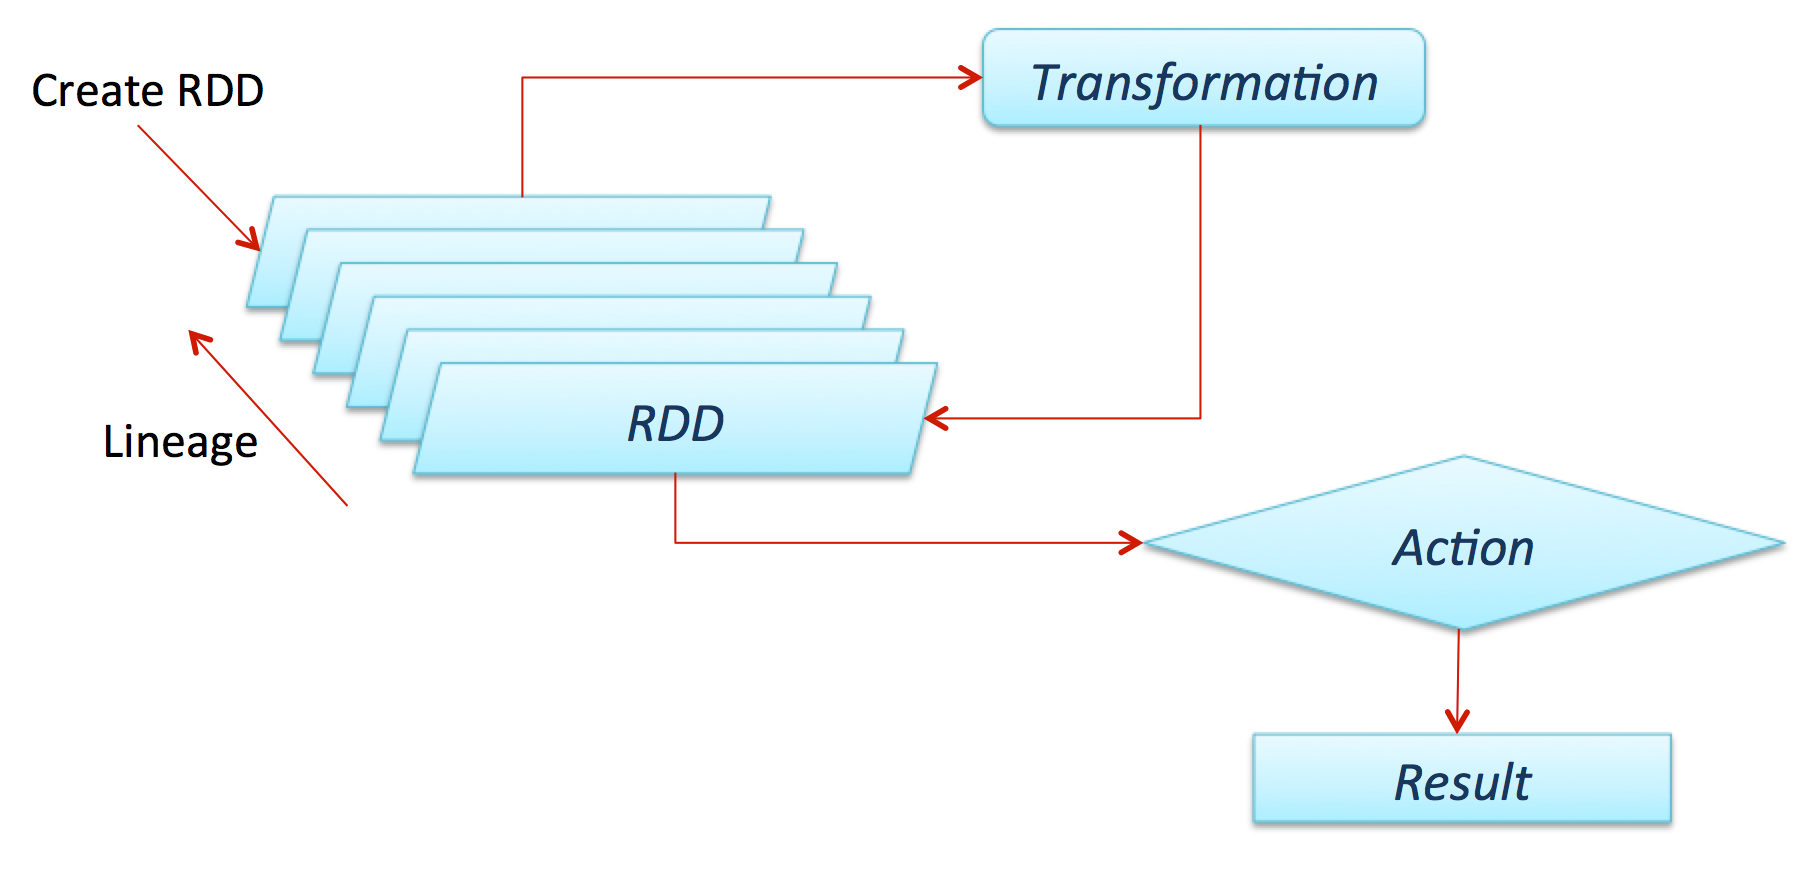
\includegraphics[width=10cm]{images/rdd_transformations.png}
\vspace{-0.2cm}
\end{figure}
\end{comment}



\-\ \\ \noindent \textbf{Helpful References:}
\begin{itemize}
    \item \textbf{Apache Spark -}  \href{https://en.wikipedia.org/wiki/Apache_Spark}{\color{blue}{https://en.wikipedia.org/wiki/Apache\_Spark}} \vspace{-0.1cm}
    \item \textbf{RDDs} - \href{https://www.tutorialspoint.com/apache_spark/apache_spark_rdd.htm}{\color{blue}{https://www.tutorialspoint.com/apache\_spark/apache\_spark\_rdd.htm}}\vspace{-0.1cm}
    \item \textbf{Spark Architecture -} \href{https://www.edureka.co/blog/spark-architecture/}{\color{blue}{https://www.edureka.co/blog/spark-architecture/}} \vspace{-0.1cm}
    \item \textbf{Spark Parallel Processing -}
    \href{https://www.simplilearn.com/spark-parallel-processing-tutorial}{\color{blue}{https://www.simplilearn.com/spark-parallel-processing-tutorial}}\vspace{-0.1cm}
    \item \textbf{Spark Examples -} \href{https://spark.apache.org/examples.html}{\color{blue}{https://spark.apache.org/examples.html}} (See Java Examples)\vspace{-0.1cm}
    \item \textbf{Spark Java API -} \href{https://spark.apache.org/docs/latest/api/java/index.html}{\color{blue}{https://spark.apache.org/docs/latest/api/java/index.html}}
\end{itemize}

\newpage

\begin{comment}
\subsection*{Processing Design}
\subsubsection*{Resilient Distributed Datasets}

Apache Spark architecture is centered around the resilient distributed dataset (RDD). Simply put an RDD is ready only (immutable) dataset. Processing of an RDD consists of transformations that take the data and create new RDDs that can further be transformed. This model allows for 
\begin{enumerate}
    \item Resiliency 
    \item Distributed Computing 
\end{enumerate}

\begin{figure}[hbt!]
\vspace{-0.0cm}
\centering
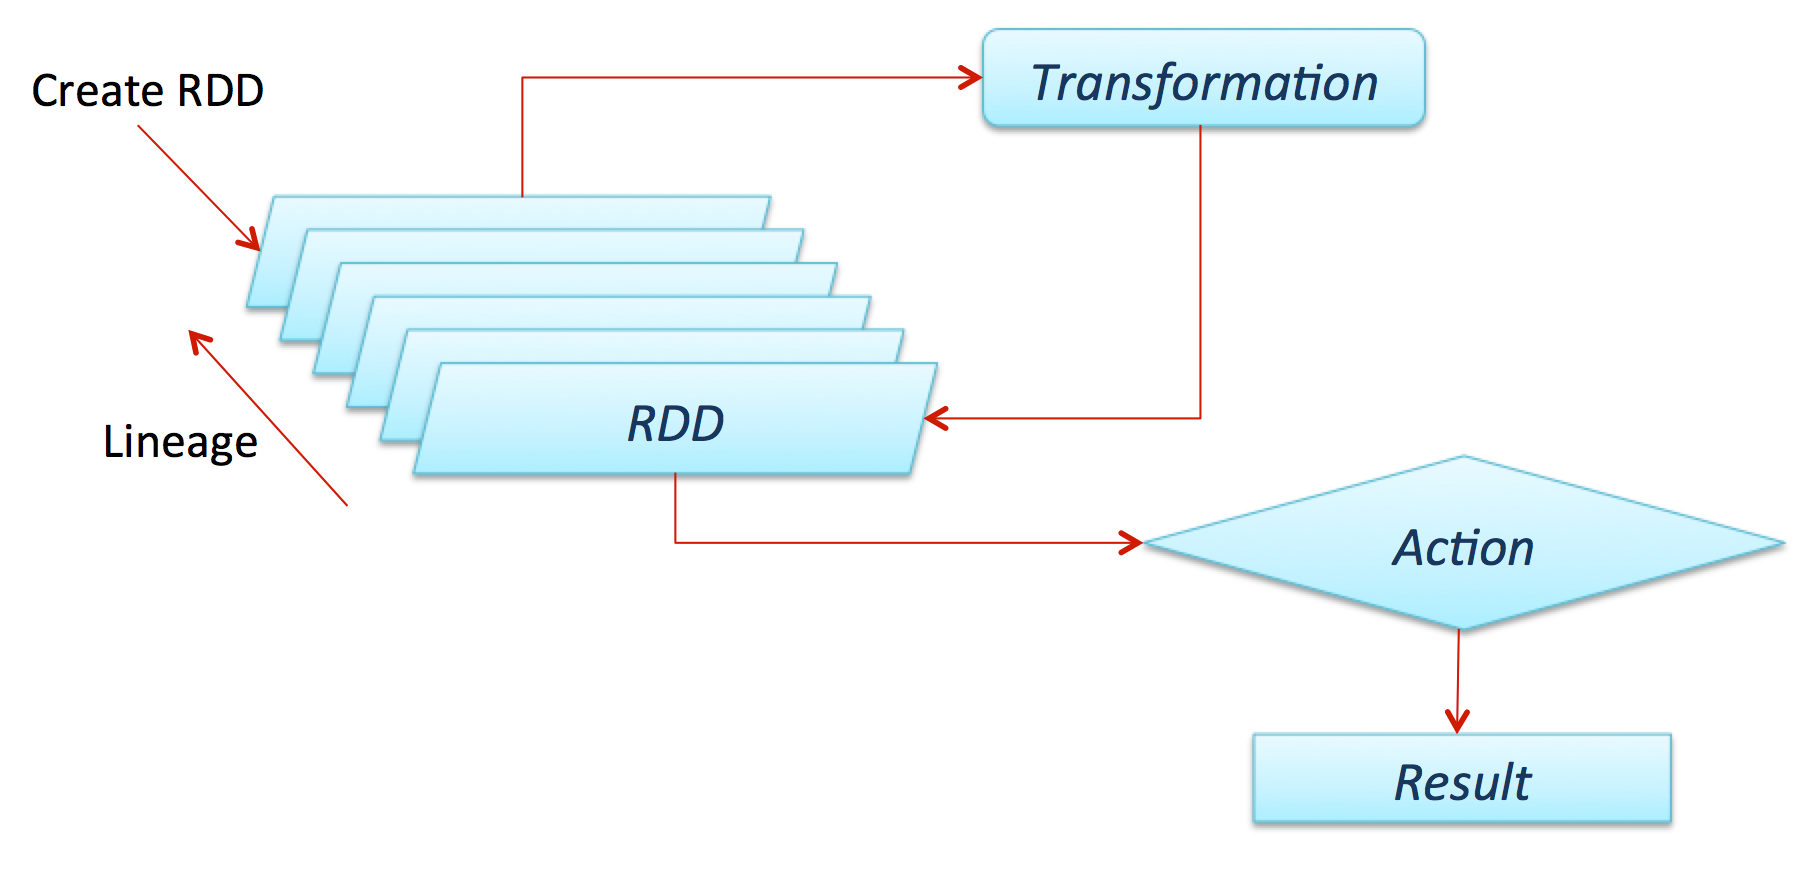
\includegraphics[width=12cm]{images/rdd_transformations.png}
\vspace{-0.2cm}
\end{figure}

\-\ \\ \noindent \textbf{You can read more about Resilient Distrbuted Datasets here:}\\
\href{https://www.tutorialspoint.com/apache_spark/apache_spark_rdd.htm}{\color{blue}{https://www.tutorialspoint.com/apache\_spark/apache\_spark\_rdd.htm}}

\subsubsection*{Transformations as a Processing Approach}
Utilizating transformations as a processing approach also gives Spark the ability to maximize parallel processing. In prior approaches such as "Map Reduce". Data sets are transformed using a set of mapping stages and reduction stages. Although each stage can be 

However in this case of Spark uses transformations, which you can think of as any operation that transforms the data (including map and reduce operations). Since these transformations are generalized, Apache Spark can actually bypass the need to synchronize between stages and carry out different parts of each transformation in parallel. 


\subsection*{Architecture}

Spark's Architecture on RDD's is important as it is able to split RDDs into multiple chunks to 

By representing data processing as a set of transformations, Spark is able to not only split RDDs to be transformed in parallel, but multiple transformations can also be carried out in parallel in a pipe lined fashion. This is comparative to a prior map-reduce approaches, where a each "mapping" operation which is a simple transformation must be done in a linear fashion. 

With this design 


\begin{figure}[hbt!]
\vspace{-0.0cm}
\centering
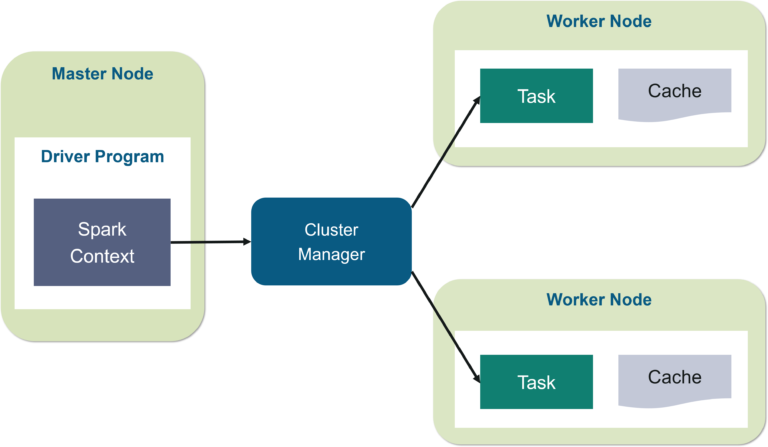
\includegraphics[width=12cm]{images/spark_arch.png}
\vspace{-0.2cm}
\end{figure}



\-\ \\ \noindent \textbf{You can read more about Spark's Architecture here:}
\href{https://www.edureka.co/blog/spark-architecture/}{\color{blue}{https://www.edureka.co/blog/spark-architecture/}}
\end{comment}






\section{Analyzing Reddit Data}
\subsection*{Intro to Reddit}
Reddit is a popular social news website where content is organized into user created boards called "subreddits". Users can add posts to subreddits.  Users can subscribe to subreddits to see new posts posted within the subreddit on their homepage. In its basic form, the homepage of Reddit would present a curated feed of popular posts among the subreddits the user is subscribed to. Each post can be "upvoted" or "downvoted". A post can be commented on and each comment can also be "upvoted" or "downvoted". An upvote and downvote can be compared to "like" and "dislike" on Facebook. A user can"upvote" a post if they believe it is contributes to the current "conversation". Likewise, users can "downvote" a post if they believe it does not contribute to the current "conversation". Through the use of upvoting and downvoting mechanisms, users help Reddit algorithms rank and determine quality content that users would be interested in.

\begin{figure}[hbt!]
\vspace{-0.0cm}
\centering

\includegraphics[width=5cm]{images/reddit-logo}
\vspace{-0.2cm}
\end{figure}

\-\\\ \noindent \textbf{Learn more about Reddit here:} \href{https://en.wikipedia.org/wiki/Reddit}{\color{blue}{https://en.wikipedia.org/wiki/Reddit}}


\subsection*{Reddit as a Basis for Social Media Research}
Within social media, certain content can be posted multiple times. In the case of Reddit, similar content can be posted multiple times in more than one subreddit. In the context of Reddit, when some content is resubmitted in another post, it is called a "repost". Analysis of reposts help provide a means in understanding social media content placement. Even though two users can submit two different posts using the same content, each post could perform differently. It becomes apparent that there is a multitude of factors that contribute to the performance of a post besides the content such as: the number of user subscribed to the subreddit, how attractive the post title is, the time of day the post was uploaded, and so on. With the large user base of Reddit along with Reddit's board system of subreddits providing simple modeling of social communities, it has been seen to be a good platform to research social media interactions, patterns, and phenomena.

\begin{comment}
Within the paper "\textit{What's in a name? Understanding the Interplay between Titles, Content, and Communities in Social Media}", researchers Lakkarajue et al. did just this. They collected Reddit data to analyze how certain factors contribute to the popularity of reposts. For their data set, they collected information on reposts of images as it was significantly easy to identify reposted images using reverse image search. Using the data set, they were able to derive models on how time, social context, and presentation affected a post's performance, ultimately helping them understand when, where, and how a post should be presented to maximize its reach.
\end{comment}

\-\ \\\textbf{You can learn more about this kind of research here:} \href{http://i.stanford.edu/~julian/pdfs/icwsm13.pdf}{\color{blue}{http://i.stanford.edu/~julian/pdfs/icwsm13.pdf}}

%----------------------------------------------------------------------------------------
%	The Task
%----------------------------------------------------------------------------------------

\subsection*{Goal:} The goal of this section is to create Spark programs to process the Reddit repost data in a way that will help us do some data analysis of our own.

\subsection*{Data Format}
Every row within the Reddit data set represents a repost of a particular photo and the format of each row is listed in \textbf{\textit{RedditData-Cols.csv}}:


\small
\begin{verbatim}
   <image id>, <unixtime>, <post title>, <subreddit>, <# upvotes>, <# downvotes>, <# comments>
\end{verbatim}
\normalsize


\noindent Provided are three different sized Reddit data files:
\begin{enumerate}
    \item \textbf{RedditData-Small.csv} - reposts of 10 unique photos ($\sim$200 rows)($\sim$16KB in size)
    \item \textbf{RedditData-Medium.csv} - reposts of 1,000 unique photos ($\sim$12k rows)($\sim$1MB in size)
    \item \textbf{RedditData-Large.csv} - reposts of 16,736 unique photos ($\sim$130k rows)($\sim$9MB in size)
\end{enumerate}

\noindent \textbf{Note:}  The small and medium data sets are simply subsets of the large data set. As you start to implement your spark programs, you should start off by running your programs on the smaller data sets then move up to the larger ones. 


\subsection{Image Impact (20 points)}
\subsubsection*{Understanding Popular Image Content:}
A photo can be reposted in multiple subreddits and the level of interactions and impact the photo has is highly dependent on which subreddit it is posted to. We can safely assume that a picture will do better in a more relevant subreddit, but what can we say about the photo in relation to the overall Reddit audience? If we post a gif of a baby elephant in multiple subreddits, would it make a bigger impact than posting a picture of a kitten in the same subreddits? \\

\noindent In this part, we want to answer the question: 

\begin{center}
    \textit{How impactful is a particular kind of photo?}
\end{center}

\begin{comment}
In this case, we want to find out what kinds of photos do better than others? This would give us some sort of idea of what the overall Reddit users 

We can than analyze the photo and context of the photo to identify particular features or topics that generate interest among Reddit users overall. 
\end{comment}


\noindent In this part we will compare images that have been reposted based on the amount of impact they had on Reddit. We can do this by measuring the amount of engagement each photo induced. This can be done by through simply counting user interactions for each photo.

\subsubsection*{Calculating Image Impact:}
As you've learned, users on Reddit can interact with posts by upvoting, downvoting, or commenting. We can simply define a post's impact to be the number of times it was upvoted, downvoted, or commented on:
$$Impact = upvotes + downvotes + comments $$
This would calculate the impact of a particular post, not a particular image. To calculate the impact of an image, we can simply extend our definition of the impact of a post to define the impact of a particular image to be the sum of all impact values for all the posts associated to a particular image:
$$Impact_{id} = \sum upvotes_p + downvotes_p + comments_p, \forall p \in P_{id} $$
In this equation, $p$ is a post within $P_{id}$, the set all of posts associated with some image with an id $id$.

\subsubsection*{Output and Analysis:}
The output of your computation should be formatted as rows where each row consists of:
\begin{lstlisting}[language=bash]
                        <image id>  <impact score>
\end{lstlisting}

\noindent \textbf{For Example:}\\
As a basic example lets say we have three entries representing three posts: 

%\begin{lstlisting}[language=bash]
\begin{Verbatim}[frame=single]
image_id, unixtime, title, subreddit, #_upvotes, #_downvotes, #_comments
123, 1733286229, A, funny, 200, 50, 6
152, 1176793353, B, cute, 350, 100, 12
123, 1559764551, C, pics, 450, 5, 12
\end{Verbatim}
%\end{lstlisting}
We can see the first and third entry are posts associated to an image with the id 123 and the second entry is a post associated with a image 152.


\-\ \\In the end, the result of our program should look like such:
%\begin{lstlisting}[language=bash]
\begin{Verbatim}[frame=single]
123 723
152 462
\end{Verbatim}
%\end{lstlisting}
From this we can see more people interacted with posts associated with the  image of id 123 compared to the posts associated with image of id 152. We could naively say the image of id 123 had more impact than the image of id 152. If image of id 123 was perhaps an image of a cat and image of id 152 was an image of a shoe, we can predict that if we posted a similar image of a cat to that in image of id 123, it could potentially be more engaging and get more exposure than if we posted a picture of a shoe similar to the image of 152.


\subsection{Repost Timing (25 points)}
\subsubsection*{Understanding Diurnal Patterns:}
Almost half of Reddit's traffic is from the United States. Given this and given the United States only spans 6 out of the $\sim$24 timezones in the world, perhaps there are some diurnal patterns that can be found with regards to post performance. A diurnal pattern is any pattern that occurs every 24 hours. One example of a potential diurnal pattern is that perhaps between 6PM and 8PM EST, Reddit posts see more interaction because a majority of users are off from work, school, etc. However our data is centered around reposts so we want to find if there are particular diurnal patterns with regards to repost performance.\\

\noindent In this part, we want to answer the question:

\begin{center}
    \textit{Is there an ideal time of the day to post a repost?}
\end{center}

\noindent In this part we will compare the hours of the day based on the amount of impact reposts posted within a particular hour had on Reddit. We can do this by measuring the amount of engagement/impact reposts posted within a particular hour had.


\subsubsection*{Calculating the Most Impactful Repost Time:}
Calculating the an hour's impact is similar to how you calculated a particular photo's impact in the previous section, except that the impact values are summed based on which hour of the day a repost was posted.

$$Impact_{hour} = \sum Impact_{p}, \forall p \in P_{hour}$$

\noindent In this equation, $p$ is a post within $P_{hour}$, the set all of posts submitted within the same hour of the day.


\subsubsection*{Output and Analysis:}
The output of your computation should be formatted as 24 rows where each row consists of:
\begin{lstlisting}[language=bash]
                    <hour offset>  <impact score>
\end{lstlisting}
where the hour offset is based on EST (the timezone Rutgers is located in). \\

\noindent \textbf{For Example:}\\
As a basic example lets say we have three entries representing three posts: 
%\begin{lstlisting}[language=bash]
\begin{Verbatim}[frame=single]
image_id, unixtime, title, subreddit, #_upvotes, #_downvotes, #_comments
123, 1616703628, A, funny, 200, 50, 6
152, 1616779228, B, cute, 350, 100, 12
123, 1616780728, C, pics, 450, 5, 12
\end{Verbatim}
%\end{lstlisting}
Here, when we convert the unix timestamps to EST, we see the first post was posted at 4:20PM EST on 3/25 and the second and third posts were posted at 1:20PM EST and 1:45PM EST respectively on 3/26.


\-\ \\In the end, the result of our program should look like such:
%\begin{lstlisting}[language=bash]
\begin{Verbatim}[frame=single]
0 0
....
13 929
....
16 256
....
23 0
\end{Verbatim}
%\end{lstlisting}
In this example output we can see that reposts submitted between 1PM-2PM EST (13th hour of the day) ended up having the most impact/reach. Perhaps we can deduce that people like to interact on Reddit when it's around lunch time, as people each typically lunch between 10AM-2PM within the United States (Remember 1-2PM EST is equivalent to 10-11AM PST). 

\begin{comment}
\vspace{-0.1cm}
\begin{info}[Remember to use EST hour offsets:]
Unixtime can represent different times of the day depending on the timezone. For this case, we want to format our results for Eastern Standard Time (EST), so sure when you're grouping the submissions to its corresponding hour offset based on EST.
\end{info}
\end{comment}

\newpage
\section{Analyzing Netflix Data}
\subsection*{Intro to Netflix}
Netflix is a popular subscription-based streaming service where users can watch and rate movies/tv shows that are present in their library of tens of thousands of titles. Users can navigate the large library of titles in multiple ways; they can search titles manually, navigate through titles within a particular category, or sift through titles that Netflix recommends them. Overall, Netflix's recommendation system is the biggest feature that sets them apart from other streaming services. By using information about the user, their watch history, and title ratings, Netflix can recommend titles that the user may like with high probability, leading to a positive platform experience. 



\begin{figure}[hbt!]
\vspace{-0.3cm}
\centering

\includegraphics[width=5cm]{images/Netflix-Logo}
\vspace{-1.2cm}
\end{figure}

\-\ \\ \\ \noindent \textbf{You can learn more about Netflix here:} \href{https://en.wikipedia.org/wiki/Netflix}{\color{blue}{https://en.wikipedia.org/wiki/Netflix}}




\subsection*{Netflix as a Basis for Developing Prediction Algorithms}
In order to maintain customers and ensure subscribers keep using their service, it is important that Netflix's recommendation and discovery mechanisms are highly effective in helping users find quality content. A large area that supports these mechanisms are predictive algorithms. Predictive algorithms use statistical analysis, machine learning, and perhaps even AI to make predictions about the future. In the context of Netflix, they want to predict what a user would rate a particular movie to help the recommendation system determine whether or not to recommend a particular title to a particular user. 

Netflix's proprietary recommendation algorithm known as \textit{CineMatch} had already been proven to be very good at predicting movies that subscribers would like. However at some point, Netflix realized that there could be better prediction algorithms out there. Because of this, they released a public data set of user reviews as part of a contest to see if people could come up with better algorithms. This contest, known as the "Netflix Prize", was held over multiple years from 2007 to 2009 and yielded algorithms and improvements that has helped Netflix's  prediction and recommendation algorithms become one of the best among streaming services today. 



\-\ \\ \noindent \textbf{You can learn more about the Netflix Prize here:} \href{https://en.wikipedia.org/wiki/Netflix_Prize}{\color{blue}{https://en.wikipedia.org/wiki/Netflix\_Prize}}


\subsection*{Goal:} The goal of this section is to create our own Spark programs to process the Netflix data set to generate some useful insights of our own.

\subsection*{Data Format}
Every row within the Netflix data set represents a movie review and the format of each row is listed in \\ \textbf{\textit{NetflixData-Cols.csv}}:

\large
\begin{verbatim}
            <movie_id>, <customer_id>, <rating>, <date>
\end{verbatim}
\normalsize


\noindent Provided are three different sized Reddit data files:
\begin{itemize}
    \item \textbf{NetflixData-Small.csv} - reviews of 10 movies ($\sim$20k rows)($\sim$450KB in size)
    \item \textbf{NetflixData-Medium.csv} - reviews of 1,000 movies ($\sim$5m rows)($\sim$120MB in size)
    \item \textbf{NetflixData-Large.csv} - reviews of 18k movies ($\sim$100m rows)($\sim$2.5GB in size)
\end{itemize}

\noindent \textbf{Note:} The small and medium data sets are simply subsets of the large data set. As you start to implement your spark programs, you should start off by running your programs on the smaller data sets then move up to the larger ones. 


\subsection{Average Movie Rating (20 points)}
\subsubsection*{Who cares about the Average Movie Rating?}
Remember the goal of any subscription-based service is user retention. The longer a user is subscribed, the more money the company gets. In the context of Netflix, if a user is happy with how and what they watch, they will most likely keep using the service in the future and maintain their subscription.

So where does the average rating fit into this? So the average rating for a movie/show fits into helping users in "how" they consume media on Netflix. Since the average rating of a movie/show is a good indicator of the quality of that movie/show with respect to the general audience, users can use these ratings to guide the way they choose the next movie or show to watch and identify whether or not a movie or television show is worth watching. 

\begin{comment}
In the end, by helping user guide the way they choose content, the average rating help users pick content that will most likely yield a positive experience. Another way to think about is that with average ratings, we can minimize the amount of disappointment a user experiences after investing a notable amount of time splurging on a movie or show.
\end{comment}

\begin{comment}
This is where the average rating for each movie/show comes in. The average rating of a movie/show is a good indicator of the quality of with respect to the general audience. 

With this, users are able to navigate the repository of movies and shows in a guided way and identify whether or not a movie/show is worth investing time into. 

Typically these are used by users to identify if a movie or television show is worth watching. We want to minimize the amount of disappointment a user takes on before investing a notable amount of time splurging on a movie or show. Thus by keeping track of the average rating for each movie will allow other users to trust and navigate the platform with better intention. 
\end{comment}


\subsubsection*{Calculating the Average Rating for a Movie:}
Although calculating average ratings for each movie is straight forward, things could be more scalable if we computed the average ratings for each movie in a distributed way. That way, if we were to get an even larger data set, the time it takes to compute the average rating for each movie wouldn't scale as linearly as if we used a single process/system.\\

\noindent Given this set of customers,  the average rating of each movie of id $id$ is the sum of all ratings for that movie divided by the number of ratings:

\vspace{0.1cm}
$$AvgRating_{id} = \frac{\sum Rating_i}{\#\ of\ ratings} \forall i \in R_{id}$$
\vspace{0.1cm}

\noindent The average rating for a movie with id $id$ would be the summation of all ratings of each review $i$ in the set $R_{id}$ which is the set of all reviews for a movie with id $id$.

\subsubsection*{Output and Analysis:}
In the end, the result of our program should be the list of all movies and their average rating in the format:
\begin{lstlisting}[language=bash]
                        <movie id> <average rating> 
\end{lstlisting}
\vspace{0.1cm}
where the average rating is truncated to 2 decimal places.\\

\noindent \textbf{For example:}\\
As a basic example lets say we have 5 reviews spanning two different movies: 
%\begin{lstlisting}[language=bash]
\begin{Verbatim}[frame=single]
movie_id, customer_id, rating, date
201, 1062, 2, 3-13-20
973, 7028, 5, 4-23-20
201, 1637, 5, 3-24-20
973, 1644, 4, 5-1-20
201, 2023, 3, 5-19-20
\end{Verbatim}
%\end{lstlisting}
We can see that three of the reviews are for movie with id X and two of the the reviews are for the movie with id Y.

\-\ \\In the end, the result of our program should look like such:
%\begin{lstlisting}[language=bash]
\begin{Verbatim}[frame=single]
201 3.33
973 4.5
\end{Verbatim}
%\end{lstlisting}
Based on the results we can see that, according to our general public sample of 5 reviews on 2 movies example, a user would probably like movie 973 compared to 201. 

\newpage
\subsection{Recommendation Graph (35 points)}
\subsubsection*{Understanding Customer Similarities:}
In the last exercise you calculated the average rating for each movie, which is a good metric to help guide Netflix users to pick content that will be of high quality to them. However, another mechanism that is typically used to guide users to quality content is a recommendation system. Recommendation systems typically take into account a user's interests, watch history, as well other user's reviews to recommend content that the user may like.

Netflix currently has their own recommendation system that millions of users are exposed to everyday. These algorithms are proprietary, but perhaps we can build towards our own recommendation system and algorithms by generating our own naive recommendation graph. 

\subsubsection*{The Recommendation Graph:}
\noindent The idea of a recommendation graph is simple. We want a graph that will encapsulate similarities between any two customers so that we can recommend content to similar customers. \\

\noindent The structure of the graph is as follows:
\begin{enumerate}
    \item A node within the graph represents a customer. 
    \item Each edge between nodes is undirected and represents similar taste between two customers of some weight. 
\end{enumerate}

\noindent To makes things simple, let us assume that two customers $A$ and $B$ have similar taste if they gave the same rating $r$ to the same movie $m$:

\begin{equation*}
Similar(A,B,m)=\begin{cases}
          1 \quad &\text{if } \, r_{m,A} = r_{m,B} \\
          0 \quad & \text{otherwise} \\
     \end{cases}
\end{equation*}
\vspace{0.1cm}

\noindent Assuming the weight of the edge between $A$ and $B$ would be the number of times $A$ and $B$ had similar tastes, then the weight of the edge between $A$ and $B$ would simply be the total number of all similar ratings:
\vspace{0.1cm}
$$EdgeWeight(A,B) = \sum Similar(A,B,m), \forall m \in M$$
\vspace{0.1cm}
where $M$ is the set of all movies.\\

\begin{figure}[hbt!]
\vspace{-0.0cm}
\centering
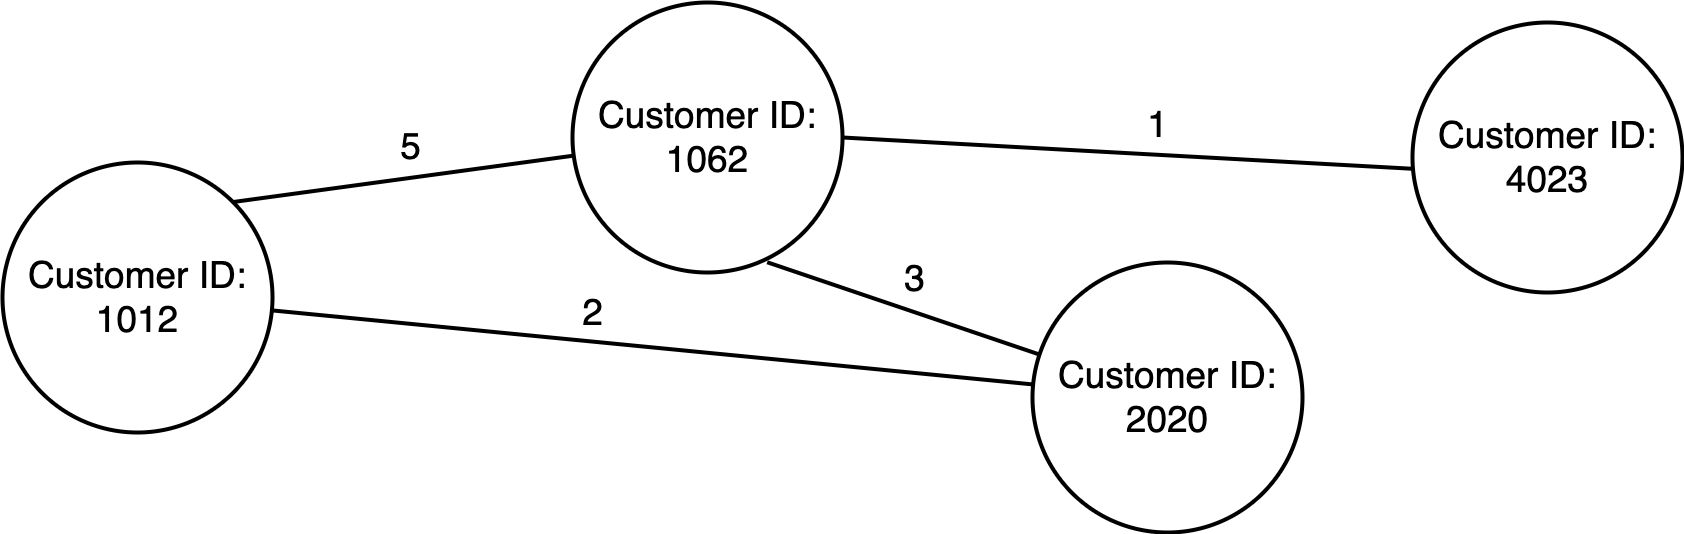
\includegraphics[width=12cm]{images/recgraph.png}
\vspace{-0.0cm}
\caption{Example Recommendation Graph}
\label{fig:recgraph}
\end{figure}



\noindent In the end, with this graph, if we find that a customer highly rated a particular movie/show, we can recommend it to their neighbors in the graph that have a high edge weight since that means they have similar tastes. 



\subsubsection*{Generating a Graph:}
Generating a graph from our data set will be a little bit more involved than our other analysis. However the main idea is that for each movie we will:
\begin{enumerate}
    \item For each (movie, rating) pair, identify the set of customers who rated the movie with that particular rating value
    \item For each (movie, rating) pair, generate an edge between each pair of customers within the set of customers that gave the movie the same rating
    \item Aggregate the edges for each customer pair to find the edge weights. 
\end{enumerate}
\begin{info}[Hint: Uniform Edges.]
Since edges are undirected, edges between customer $A$ and $B$ can take the form $(A,B)$ or $(B,A)$. However this could lead to some issues when aggregating edges since there are two possible forms to consider. To mitigate this issue and ensure edges maintain a single form between any two customers, format the edge in such a way where the first customer id of is always less than the second customer id, as shown in the example output in the next section. 
\end{info}

\subsubsection*{Output and Analysis:}
In the end, the result of our program should be a list of all the weighted edges in our graph in the format:
\begin{lstlisting}[language=bash]
                (<customer_id_1>, <customer_id_2>) <weight> 
\end{lstlisting}
where \textit{customer\_id\_1} is less than \textit{customer\_id\_2}.\\

\noindent \textbf{For example:}\\
The output for the graph in Figure~\ref{fig:recgraph} would look something like:
%\begin{lstlisting}[language=bash]
\begin{Verbatim}[frame=single]
(1012,1062) 5
(1012,2020) 2
(1062,2020) 3
(1062,4023) 1
\end{Verbatim}
%\end{lstlisting}
Here we can see that customer 1012 has 5 similar ratings to 1062. So, if customer 1012 highly rates a movie/show, we can recommend that movie/show with relatively high confidence to customer 1062 and vice versa. 

\section{Getting Started}

\subsection{Project Template Overview}

The following is the bare structure of the project template: \\

\dirtree{%
.1 project-template.
.2 src.
.3 main.
.4 java.
.5 com.
.6 RUSpark.
.7 WordCount.java.
.7 RedditPhotoImpact.java.
.7 RedditHourImpact.java.
.7 NetflixMovieAverage.java.
.7 NetflixGraphGenerate.java.
.2 pom.xml.
}

\begin{info}[Notice:]
If you imported the project into Eclipse, additional folders may be present. This is due to Eclipse realizing that it is a Maven project, auto generating extra folders that it may use.
\end{info}

\noindent \textbf{\underline{Main Implementation Files}} \vspace{0.2cm} \\
\noindent Within the /src/main/java/com/RUSpark directory the five main Java files:
\begin{itemize}
   \item \textbf{\textit{WordCount.java}} - This is an example Spark program that counts the numbers of occurrences of each word in a text file.
    \item \textbf{\textit{RedditPhotoImpact.java}} - This is where you will implement the Spark program that calculates the impact of every photo within the Reddit data set
    \item \textbf{\textit{RedditHourImpact.java}} - This is where you will implement the Spark program that calculates the impact of all posts submitted within the same hour of the day
    \item \textbf{\textit{NetflixMovieAverage.java}} - This is where you will implement the Spark program that calculates the average rating of all movies within the Netflix data set 
    \item \textbf{\textit{NetflixGraphGenerate.java}} - This is where you will implement the Spark program that generates a recommendation graph as a list of weighted edges between customers
\end{itemize}

\noindent \textbf{\underline{Pom Configuration File}} \vspace{0.2cm} \\
\noindent Lastly, you will notice at the root of the project there is a file called \textbf{\textit{pom.xml}}. This file is for Maven. Like mentioned in the previous section notice, Maven is a build tool used for Java projects and uses the pom.xml file to know how to build the Java project as well as know what dependencies need to downloaded before hand. \textbf{DO NOT EDIT THIS FILE}. The pom.xml file has been preconfigured to generate Runnable JARs every time the project is compiled \textit{for your convenience}. 



\subsection{Reddit Dataset}

\subsubsection*{Contents and Description:}
The Reddit Dataset (\textbf{\textit{RedditData.zip}}) includes the following files:
\begin{itemize}
    \item \textit{\textbf{RedditData-Cols.csv}} - file of column names (1 row) ($\sim$100B in size)
    \item \textit{\textbf{RedditData-Small.csv}} - reposts of 10 unique photos ($\sim$200 rows)($\sim$16KB in size)
    \item \textit{\textbf{RedditData-Medium.csv}} - reposts of 1,000 unique photos ($\sim$12k rows)($\sim$1MB in size)
    \item \textit{\textbf{RedditData-Large.csv}} - reposts of 16,736 unique photos ($\sim$130k rows)($\sim$9MB in size)
\end{itemize}

\subsubsection*{Data Format:}
Every row within the Reddit Data represents a repost and the format of each row is listed in \\ \textbf{\textit{RedditData-Cols.csv}}:
\small
\begin{verbatim}
   <image id>, <unixtime>, <post title>, <subreddit>, <# upvotes>, <# downvotes>, <# comments>
\end{verbatim}
\normalsize

\subsubsection*{Space Requirements:}
The compressed dataset (\textbf{\textit{RedditData.zip}}) is appoximately $\sim$4MB in size and uncompressed is around $\sim$10MB, so make sure you have about $\sim$15MB of free space when downloading.

\subsubsection*{Downloading the Dataset:}
\begin{itemize}
    \item \textbf{Via Web Browser:}\\
        To download the data set from a browser, use the following link:
        \begin{center}
        \href{https://drive.google.com/uc?export=download&id=1zhtVn8-64QKpjl_y0uHWImooeSJkv7bc}{\color{blue}{https://drive.google.com/uc?export=download\&id=1zhtVn8-64QKpjl\_y0uHWImooeSJkv7bc}}
        \end{center}
    \item \textbf{Via Command Line (WGET):}\\
        To download the dataset using \textit{wget}, copy and paste the following command and run it:
        \begin{commandline}\begin{verbatim}$ wget -O RedditData.zip "https://docs.google.com/uc?export=download&id=
"1zhtVn8-64QKpjl_y0uHWImooeSJkv7bc\end{verbatim}\end{commandline}
    \item \textbf{Via Command Line (CURL):}\\
        To download the dataset using \textit{curl}, copy and paste the following command and run it:
        \begin{commandline}\begin{verbatim}$ curl -L -o RedditData.zip "https://drive.google.com/uc?export=download
&id="1zhtVn8-64QKpjl_y0uHWImooeSJkv7bc\end{verbatim}\end{commandline}
\end{itemize}

\subsubsection*{Extracting the Dataset:}
To extract the dataset, simply use the \textit{unzip} command:
\begin{commandline}\begin{verbatim}$ unzip RedditData.zip\end{verbatim}\end{commandline}



\subsection{Netflix Dataset}

\subsubsection*{Contents and Description:}
The Netflix Dataset (\textbf{\textit{NetflixData.zip}}) includes the following files:
\begin{itemize}
    \item \textit{\textbf{NetflixData-Cols.csv}} - file of column names (1 row) ($\sim$30B in size)
    \item \textit{\textbf{NetflixData-Small.csv}} - reviews of 10 movies ($\sim$20k rows)($\sim$450KB in size)
    \item \textit{\textbf{NetflixData-Medium.csv}} - reviews of 1,000 movies ($\sim$5m rows)($\sim$120MB in size)
    \item \textit{\textbf{NetflixData-Large.csv}} - reviews of 18k movies ($\sim$100m rows)($\sim$2.5GB in size)
    \item \textit{\textbf{NetflixData-Titles.csv}} - list of movie indexes and titles ($\sim$18k rows)($\sim$600KB in size)
\end{itemize}

\subsubsection*{Data Format:}
Every row within the Netflix Data represents a movie review and the format of each row is listed in \\ \textbf{\textit{NetflixData-Cols.csv}}:

\large
\begin{verbatim}
           <movie id>, <customer id>, <rating>, <date>
\end{verbatim}
\normalsize

\subsubsection*{Space Requirements:}
The compressed dataset (\textbf{\textit{NetflixData.zip}}) is appoximately $\sim$700MB in size and uncompressed is around $\sim$2.6GB, so make sure you have about $\sim$3.5GB of free space when downloading.


\subsubsection*{Downloading the Dataset:}
\begin{itemize}
    \item \textbf{Download via Browser:}\\
        To download the data set from a browser use the following link:
        \begin{center}
        \href{https://drive.google.com/uc?export=download&id=1RcLSh1EuY5iL48ldqiTYfZaM7zw7KASi}{\color{blue}{https://drive.google.com/uc?export=download\&id=1RcLSh1EuY5iL48ldqiTYfZaM7zw7KASi}}
        \end{center}
    \item \textbf{Via Command Line (WGET):}\\
        To download the dataset using \textit{wget}, copy and paste the following command and run it:
        \begin{commandline}\begin{verbatim}$ wget --save-cookies cookies.txt "https://docs.google.com/uc?export=dow
nload&id="1RcLSh1EuY5iL48ldqiTYfZaM7zw7KASi -O- | sed -rn "s/.*confirm=(
[0-9A-Za-z_]+).*/\1/p" > confirm.txt; wget --load-cookies cookies.txt -
O NetflixData.zip "https://docs.google.com/uc?export=download&id="1RcLSh
1EuY5iL48ldqiTYfZaM7zw7KASi"&confirm="$(<confirm.txt); rm -f confirm.tx
t cookies.txt\end{verbatim}\end{commandline}
    \item \textbf{Via Command Line (CURL):}\\
        To download the dataset using \textit{curl}, copy and paste the following command and run it:
        \begin{commandline}\begin{verbatim}$ curl -L -c cookies.txt "https://docs.google.com/uc?export=download&id=
"1RcLSh1EuY5iL48ldqiTYfZaM7zw7KASi | sed -rn "s/.*confirm=([0-9A-Za-z_]+
).*/\1/p" > confirm.txt; curl -L -b cookies.txt -o NetflixData.zip "http
s://docs.google.com/uc?export=download&id="1RcLSh1EuY5iL48ldqiTYfZaM7zw7
KASi"&confirm="$(<confirm.txt); rm -f confirm.txt cookies.txt\end{verbatim}
\end{commandline}
\end{itemize}

\subsubsection*{Extracting the Dataset:}
To extract the dataset, simply use the \textit{unzip} command:
\begin{commandline}\begin{verbatim}$ unzip NetflixData.zip\end{verbatim}\end{commandline}




\subsection{Building the Project}
To build your project, you will need to use Maven and run "goals". Goals are procedures that carry out actions related to the project lifecycle. There are three Maven goals you will need will to familiarize yourself with in order to build and compile your project:
\begin{itemize}
\item install - this goal downloads any dependencies for your project
\item package - this goal compiles the project and packages artifacts
\item clean - this goal cleans the project of any artifacts and code generated by the project
\end{itemize}

\subsubsection*{Install}
The install goal downloads any dependencies and plugins you will need for your project. You will need to run this goal when you first import your project so the necessary Apache Spark libraries can be downloaded. If you don't do this, your IDE may give you errors or you may get errors when you try and build the project. 
\begin{itemize}
\item To do this in Eclipse:
	\begin{enumerate}
	\item In Eclipse, select the project folder within the Package Explorer window.
	\item Go to "Run" > "Run As" > "Maven Install"
	\end{enumerate}
\item To do this in Command Line:
	\begin{enumerate}
	\item Navigate to the root of the project directory.
	\item Run the following: "mvn install"
	\end{enumerate}
\end{itemize}

\subsubsection*{Package}
The package goal will carry out the Maven build process: compiling project code, packaging artifacts, as well as carry out any additional tasks defined within the pom.xml file. You will need to run this goal for two reasons. The first is to generate gRPC Java code. Within the pom.xml there is a task that invokes the Google Protocol Buffer compiler to take the proto file you defined and generate Java classes. These classes are what you will use to implement your service. The second reason to run the package goal is to compile your server and client code so that you can run them.
\begin{itemize}
\item To do this in Eclipse:
	\begin{enumerate}
	\item In Eclipse, select the project folder within the Package Explorer window.
	\item Go to "Run" > "Run As" > "Maven build..."
	\item Within the Goals text box, type in "package"
	\item Click "Run" 
	\end{enumerate}
\item To do this in Command Line:
	\begin{enumerate}
	\item Navigate to the root of the project directory.
	\item Run the following: "mvn package"
	\end{enumerate}
\end{itemize}

\subsubsection*{Clean}
The clean goal will clean the project directory of any generated project artifacts and source code. Project artifacts and generated code are usually placed within a folder named "target". You will need to run the clean goal before you build your project with the package goal to ensure any files from your old code is gone. You can run the package goal without running the clean goal as it will just overwrite the existing files, but there may be some files that were not overwritten still lying around.
\begin{itemize}
\item To do this in Eclipse:
	\begin{enumerate}
	\item In Eclipse, select the project folder within the Package Explorer window.
	\item Go to "Run" > "Run As" > "Maven clean"
	\end{enumerate}
\item To do this in Command Line:
	\begin{enumerate}
	\item Navigate to the root of the project directory.
	\item Run the following: "mvn clean"
	\end{enumerate}
\end{itemize}
\begin{info}[Note:]
Sometimes when running the previous goals in Eclipse, it may seem like nothing changed within the project structure. An example would be the target folder not showing up after you built your project. This is because Eclipse may have failed to update the window to reflect the new files. If this happens, try refreshing by right-clicking the project folder and selecting refresh. 
\end{info}


\subsection{Running the Project}
After compiling your project, there will be generated jars within the \textit{/target} folder within the project directory. These *.jar files are the compiled Spark programs that you will submit to the Spark cluster to run. 

\subsubsection*{Program Usage}
To run a Spark program on a Spark cluster, you will have to use the \textit{spark-submit} command to submit a *.jar Spark program to run. Each program in this project is structured to take in a single argument which specifies the data set to process. Thus the usage is as follows:

\vspace{0.1cm}
\begin{lstlisting}[language=bash]
        spark-submit  <path to Spark program>  <path to data set>
\end{lstlisting}
\vspace{0.1cm}

\noindent \textbf{For example:}
\begin{commandline}
\begin{verbatim}$ spark-submit RedditPhotoImpact.jar /common/users/djd240/RedditData-Large.csv
\end{verbatim}
\end{commandline}

\subsubsection*{Available Spark Clusters:}
You can run your project in two different places:
\begin{enumerate}
    \item \textbf{The iLab Machines}\\ 
    The iLab machines at Rutgers are equipped with Spark running in standalone mode. To run your program: (1) Ensure your compiled jar and data set are uploaded and present on the iLab machine then (2) invoke the spark-submit command like shown above. 
    \item \textbf{Amazon Web Services}\\
    If you haven't already used AWS, this could be a great opportunity to understand how AWS works. To learn how to run set up a Spark cluster on AWS and run your project take a look at the following guide here: \href{https://github.com/DaveedDomingo/Spark-Reddit-Netflix-Project/blob/main/SparkOnAWS.pdf}{\color{blue}{https://github.com/DaveedDomingo/Spark-Reddit-Netflix-Project/blob/main/SparkOnAWS.pdf}}
\end{enumerate}


\begin{info}[Note on large data sets on iLab machines:]
The data sets within this project are somewhat large. By default on the iLab machines, you have approximately $\sim$6GB of storage in your home directory (\texttt{/ilab/users/<your netid>}). However this may not be enough space. There is another filesystem where you have more space located at (\texttt{/common/users/<your netid>}). In this file system you have approximately $\sim$100GB of storage space available to you. This should be enough to store anything that won't fit in your home directory. \textbf{If using the iLab machines for this project, I recommend you download the data sets directly to your \texttt{/common/users/<your netid>} directory to ensure you don't take up space in your main home directory}. For more details on all the iLab storage options, see here: \href{https://resources.cs.rutgers.edu/docs/file-storage/storage-technology-options/}{\color{blue}{https://resources.cs.rutgers.edu/docs/file-storage/storage-technology-options/}}
\end{info}

\begin{info}[Saving Output to File:]
So the results of your program should print out in STDOUT. However you'll notice when running your Spark program, you'll also see output given from spark. You can save and isolate your output by redirecting it to a file like:
\begin{verbatim}               $ spark-submit myjar.jar inputdata.csv > out.txt
\end{verbatim}


\end{info}



\section{Recommended Steps}
The hardest part would be to learn how Apache Spark works. I recommend spending a good amount of time in the beginning to fully understand Apache Spark and try and get an test Spark program working before working on any of the parts of this project:

\begin{enumerate}
    \item Read and learn about Apache Spark 
    \item Take a look a word count example and get it running on the iLab Machines and AWS 
    \item Implement Reddit Data programs 
    \item Implement Netflix Data programs
    \item Write Writeup 
    \item Submit on time
\end{enumerate}

\section{Submission}
To submit your project, submit the following items:

\begin{enumerate}
\item \textbf{The following raw files:}
    \begin{itemize}
        \item RedditPhotoImpact.java
        \item RedditHourImpact.java
        \item NetflixMovieAverage.java
        \item NetflixGraphGenerate.java
    \end{itemize}
\item \textbf{A pdf document consisting of the following things:}
	\begin{itemize}
	\item A few pages describing your implementation and analysis:
	\begin{itemize}
	    \item For each program, describe what transformations you did to get to the result.
	    \item Based on the result from RedditPhotoImpact, what was the most impactful photo for the whole data set?
	    \item Based on the result from RedditHourImpact, what hours of the day (in EST) did submitted posts have the most impact/reach?
	    \item Based on the result from NetflixMovieAverage, name 2-3 movies that had the highest average rating.
	    %\item Based on the result from NetflixGraphGenerate, name 2-3 movies that had the highest average rating.
	\end{itemize}
	\item  Finally, a couple of paragraphs of reflection describing: What was the hardest parts about implementing your project and how did you overcome them? If you had difficulties and couldn't finish the project, describe what you think you could've done better or what you think would've helped. 
	\end{itemize}
\end{enumerate}

\noindent \textbf{Please follow all submission guidelines. Failure to do so will result in points being taken away.}

\begin{info}[Don't slack on the doc.]
The write up is very important when it comes to evaluating your project. Not only does it help us understand your approach and how your implementation works, it also shows us the amount of effort you put into the project. The write up also helps us survey the amount of effort needed to complete the project as well as gauge the project's overall difficulty. Because of these things, the write up in general allows for as much partial credit as possible as well as reasonably scaling grades across all submissions.
\end{info}

\section{Additional Tips and Tricks} % Numbered section
\begin{info}[When in doubt, Google (\textit{responsibly}):]
If you have an issue or your program is throwing an error that you don't know how to fix, Google It. Someone, somewhere, probably faced the same issue at some point. However do so responsibly and don't cheat. If you are caught cheating, your case will be handled according to Rutgers' academic integrity policy (\href{http://academicintegrity.rutgers.edu/}{http://academicintegrity.rutgers.edu/}).
\end{info}
\begin{info}[Combining Maven Goals:]
You may find yourself running Maven goals frequently to build the project. You might find yourself running them so frequently it may just interfere with your precious development time. Luckily you can group goals together. For example, since it is good practice run the clean goal before the package goal, we should group them. In Eclipse this is done by running a Maven build like we are running the package goal, but instead of writing "package" in the Goals text box, we write "clean package". In Command Line, this is done by navigating the root of the project directory and running "mvn clean package". These will both run the clean goal first then the package goal. 
\end{info}

\section*{Frequently Asked Questions}
\begin{itemize}
\item \textbf{Can I use external libraries other than the built in java libraries in my implementations?} No. You may only use the standard Java Libraries and anything else within the Apache Spark libraries.
\item \textbf{Can I use helper methods in my implementations?} Yes, as long as the program works. 
\item \textbf{Can I make other java files to support my implementation?} No, please only write your implementation within the supplied template java files.
\item \textbf{Can we implement the programs on my own computer?} Yes, as long as it can compile and run on the iLab machines as that is where they will be compiled, ran, and graded. 
\end{itemize}


\section*{Additional Questions} % Numbered section
If you have any questions about the project or are having any issues, email me at David.Domingo@rutgers.edu




\end{document}
